
\subsection{User Profiling for Travel Preferences}

In 2018, Lim et al.\cite{Lim2018a}  demonstrated how implementing
personalisation in their algorithm, which they called PersTours, helped their
algorithm to portray 
real-life scenarios more accurately. The authors built a system where the
tourist's level of interest in a specific category is dependant on their time
spent at such POIs, relative to the average user. They gathered information
from the user's past trips from the social media platform Flickr.


Nguyen et al.\cite{Nguyen2018} produced an android chat application called STSGroup that
gathers user's preferences and resolves conflicts between tourists by
understanding the messages sent in a group chat. They provided an example of
students travelling to South Tyrol (Italy), which gathered information such as
the users' mood and recommended POIs from their conversations. Other users in
the group chat rate their suggestions through a voting system as the system
uses raking lists and logistics to calculate the ideal group preferences in the
background. 

The average internet user has gone from being a passive content absorber to a
content producer through the rise in social media~\cite{Ikeda}. TTDP RSs can
use this as an advantage and provide a fully automated activity plan based on
the user's characteristics. This section describes several methods for user
profiling and information gathering from the user's social media.


\subsubsection{User Profiling based on natural language processing}

In 2013, A sentiment analysis by Ikeda et al.~\cite{Ikeda} based on a hundred thousand
Japanese user profiles managed to perform a demographic estimation. This study
shows how social media posts can be helpful to gather information about a user,
and in fact, Hung et al.\cite{Hung2008} demonstrated a user profiling
technique based on tag correlation.

\subsubsection{User Profiling based on images}

Instagram has a significant influence on the tourism industry. Sharing photos
of amazing sights and landscapes have impacted the way people
choose their POIs\cite{Terttunen2017}. Therefore, a system that uses
tourist's social media photos could impact automatic user preference gathering. 

Chen et al.\cite{Chen2013} produced a system for automatically retrieving tags
from images and incomplete tags called \emph{FastTag}. The algorithm can be
trained in \(O(n)\) time and uses two simple linear mappings. Figure
~\ref{fasttag} shows an example of an input image used alongside the incomplete
input tags \emph{snow, lake, feet}. Given these two inputs, the algorithm
produced the following additional tags, {mountain, water, legs, boat, trees}.

\begin{figure}[h]
\centering
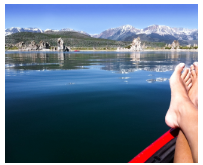
\includegraphics[width=0.2\textwidth]{Fastag}
\caption{Example of an image input for the FastTag algorithm}
\label{fasttag}
\end{figure}

Images classification techniques could provide a preference gathering system.
Deep neural networks play an essential role in this field of Image
Classification \cite{Balaji2019, Cufoglu}. We will describe how this technology
could gather information for a tourist's user preferences in the upcoming
sections.
